\section{}
\textbf{Suppose that a star is made of ideal gas, is dominated by radiative heat transfer, and is in hydrostatic equilibrium. Furthermore, the specific (per unit mass) energy generation, mean molecular weight, and opacity are the same throughout this star.
Neglecting radiation pressure, please show that the star is a polytrope of index $n = 3$.}

A polytrope is a power law stellar model for which the pressure, $P$, only depends on the density, $\rho$, as
\begin{equation}
    P = K \rho^{1 + 1/n}
    \label{eq:polytrope}
\end{equation}
where $K$ is a constant,  and $n$ is the polytrope index. 

For a star dominated by radiative heat transfer, 
\begin{equation*}
    \nabla = \frac{\partial ln T}{\partial ln P} = \frac{P \partial T}{T \partial P} = \frac{3}{4\pi ac}\frac{P\kappa}{T^4}\frac{L_r}{GM_r}
\end{equation*}
Given that the generation rate is constant then $L_r= \varepsilon M_r$ so that 
\begin{align*}
     \frac{P \partial T}{T \partial P} &= \frac{3}{4\pi ac}\frac{P\kappa}{T^4}\frac{L_r}{GM_r} = \frac{3}{4\pi ac}\frac{P\kappa}{T^4}\frac{\varepsilon M_r}{GM_r} = \frac{3}{4\pi ac}\frac{P\kappa}{T^4}\frac{\varepsilon }{G}\\
     \frac{dT}{dP} &= \frac{3}{4\pi ac}\frac{\kappa}{T^3}\frac{\varepsilon }{G}
\end{align*}

This is a differential equation that can be solved by
\begin{align*}
    \int_T T^3dT = \frac{3\kappa\varepsilon}{4\pi Gac}\int_P dP\\
    \frac{T^4}{4} = \frac{3\kappa\varepsilon}{4\pi Gac}P\\
    T^4 = \frac{3\kappa\varepsilon}{\pi Gac}P \numberthis\label{eq:Temp4}
\end{align*}

Since the star is an ideal gas $P = \rho N_A k_B T / \mu$ then we can find that $T= P \mu / (\rho N_A k_B)$ and substituting on Eq. \ref{eq:Temp4}, we find that
\begin{align*}
    \left(\frac{P\mu}{\rho N_A k_B}\right)^4 &= \frac{3\kappa\varepsilon}{\pi Gac}P \\
    P^3 &= \frac{3\kappa\varepsilon}{\pi Gac}\left(\frac{\rho N_A k_B}{\mu}\right)^{4} = \frac{3\kappa\varepsilon}{\pi Gac}\left(\frac{N_A k_B}{\mu}\right)^{4} \rho^4\\
    P &= \left(\frac{3\kappa\varepsilon}{\pi Gac}\right)^{1/3}\left(\frac{N_A k_B}{\mu}\right)^{4/3}\rho^{4/3}\numberthis\label{eq:poly4/3}
\end{align*}

Comparing Eq. \ref{eq:poly4/3} to Eq.\ref{eq:polytrope} we can see that it is a polytrope with index $n = 3$ and with constant
\begin{equation*}
    K = \left(\frac{3\kappa\varepsilon}{\pi Gac}\right)^{1/3}\left(\frac{N_A k_B}{\mu}\right)^{4/3}
\end{equation*}

%==============================================================
\Needspace{6\baselineskip}
\section{}
\textbf{Use some decent integrator to construct a polytrope with index $n = 3$.
The simplest method is to shoot for a solution. 
Please a) plot $\theta_3$ as a function of $\xi$ and b) calculate $\xi_1$, $-\theta_3^\prime(\xi_1)$, and $\rho_c/\langle\rho\rangle$ and check your results with Table 7.1 in HSK.}

To find a solution we start with Lane-Emden Equation given by 
\begin{equation*}
    \frac{1}{\xi^2}\frac{d}{d\xi}\left(\xi^2\frac{d\theta_n}{d\xi}\right) = -\theta_n^n
\end{equation*}
Following the textbook, we can do the substitutions $x=\xi$, $y=\theta_n$ and $z=y^\prime=dy/dx$, then Lane-Emden equation gets into
\begin{align*}
    \frac{1}{x^2}\frac{d}{dx}\left(x^2 z\right) = -y^n \\
    \frac{1}{x^2}(2xz + x^2z^\prime) =  -y^n \\
    z^\prime = -y^n - \frac{2z}{x} \numberthis \label{eq:LaneEmden}
\end{align*}

We can solve this equation for several values of n, including $n=3$ by using a 4th order Runge Kutta (RK4) method. The RK4 gives the corresponding values of x, y, and z for each step and stops after crossing $\theta_n=0$ line.
Figure \ref{fig:LaneEmdenSolutions} was created by plotting the x and y array given by the RK4 method, which correspond to $/xi$ and $\theta_n$, respectively.

To calculate $\xi_1$ we need to find the value of x when $y=0$, in other words, when $\theta_n(\xi_1)=0$. To do so, we did an interpolation using the values before and after it crosses the zero line. We repeat this process to find the values of z for which $y=0$ which would give us $\theta_n^\prime (\xi_1)$ since they should happen during the same step. These values can be seen in Table \ref{tab:LaneEmdenSolutions} and be compared to the solutions given by table 7.1 of the textbook. Note that this solutions are similar for both the RK4 method solution and the textbook table. 
  

\begin{figure}
    \centering
    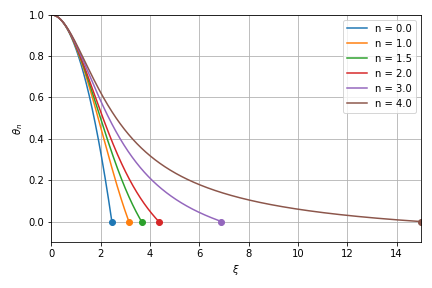
\includegraphics{CodeAndFigures/Astro643Hw3P2Plot.png}
    \caption{Solutions for polytropes with index values $n=0,1,1.5,2,3,4$ where the fill circles mark the position of $\xi_1$ defined by $\theta_n(\xi_1)=0$ and whose value can be seen on Table \ref{tab:LaneEmdenSolutions}.}
    \label{fig:LaneEmdenSolutions}
\end{figure}

\begin{table}[ht]
    \centering
    \begin{tabular}{rrrrrr}
\toprule
    n &  $\xi_1$ &  $\xi_1$ True &  $-\theta_n^\prime(\xi_1)$ &  $-\theta_n^\prime(\xi_1)$ True &  $\frac{1}{3}\left(\frac{\xi}{-\theta_n^\prime}\right)_{\xi_1}$ \\
\midrule
0.000 &    2.450 &         2.449 &                      0.817 &                           0.816 &                                              1.000 \\
1.000 &    3.142 &         3.142 &                      0.318 &                           0.318 &                                              3.291 \\
1.500 &    3.654 &         3.654 &                        NaN &                           0.203 &                                                NaN \\
2.000 &    4.353 &         4.353 &                      0.127 &                           0.127 &                                             11.404 \\
3.000 &    6.897 &         6.897 &                      0.042 &                           0.042 &                                             54.186 \\
4.000 &   14.972 &        14.972 &                      0.008 &                           0.008 &                                            622.465 \\
\bottomrule
\end{tabular}

    \caption{Solutions for polytropes with index values $n=0,1.5,1,2,3,4$ where the columns ending with "True" are the values given in Table 7.1 of the textbook and are included for comparison.}
    \label{tab:LaneEmdenSolutions}
\end{table}


%==============================================================
\Needspace{6\baselineskip}
\section{}
\textbf{Estimate the Chandrasekhar's mass of a zero temperature white dwarf, when electrons become extreme relativistic degenerate.}
\subsection{}
\textbf{Show that the equation of state can be expressed as $P=K\rho^{4/3}$ where
\begin{equation*}
    K = \frac{1}{4}\left(\frac{8\pi}{3}\right)^{-1/3}\frac{hc}{(m_A\mu_e)^{4/3}}
\end{equation*}
in which $\mu_e$ is the mean molecular weight of electrons.}

From Equation 3.53 from the textbook, we have that the pressure for degenerate electronc gas is given by
\begin{equation*}
    P_e = \frac{8\pi}{3}\frac{m_e^4c^5}{h^3}\int^{x_F}_0\frac{x^4}{(1+x^2)^{1/2}}dx = \frac{\pi}{3}\left(\frac{h}{m_ec}\right)^{-3}m_ec^2 f(x)
\end{equation*}
where $f(x)=2x^4 + 2x^2 + ... $ for relativistic electrons and 
\begin{equation*}
    x = \left(\frac{\rho}{\mu_eB}\right)^{1/3} = \left(\frac{3 N_A \rho}{8\pi \mu_e}\right)^{1/3}\frac{h}{m_ec}
\end{equation*}

Using only the first term of $f(x)$, then we have 
\begin{align*}
    P_e = \frac{\pi}{3}\left(\frac{h}{m_ec}\right)^{-3}m_ec^2 2\left( \left(\frac{3 N_A \rho}{8\pi \mu_e}\right)^{1/3}\frac{h}{m_ec}\right)^4 = \frac{3^{1/3}ch\rho^{4/3}N_A^{4/3}}{8^{1/3}\pi^{1/3}\mu_e^{4/3}} = \frac{1}{4}\left(\frac{3}{8\pi}\right)^{1/3}\frac{hc}{(m_A\mu_e)^{4/3}}\rho^{4/3} = K \rho^{4/3}
\end{align*}
where we have used $N_A = 1/m_A$. 



\subsection{}
\textbf{Show the mass of the white dwarf in this extreme is independent of the radius
R and can be expressed as
\begin{equation*}
    M = \frac{1}{4\pi}\left(\frac{3}{2}\right)^{1/2}\left(\frac{hc}{Gm_A^{4/3}}\right)^{3/2}\frac{\xi_1^2\left(-\frac{d\theta_3}{d\xi}\right)_{\xi_1}}{\mu_e^2},
\end{equation*}
where the values of $\xi_1$ and $\left(-\frac{d\theta_3}{d\xi}\right)_{\xi_1}$ can be obtained from Table 7.1.}

We can relate the constant $K$ with the mass by using Eq. 7.40 from the textbook:
\begin{equation}
    K = \left[\frac{4\pi}{\xi^{n+1}(-\theta^\prime_n)^{n-1}}\right]^{1/n}_{\xi_1}\frac{G}{n+1}M^{1-1/n}R^{-1+3/n}
    \label{eq:polytropeK}
\end{equation}

Evaluating the last equation for $n=3$ and solving for the mass, we have
\begin{align*}
    K = \left[\frac{4\pi}{\xi^{4}(-\theta^\prime_3)^{2}}\right]^{1/3}_{\xi_1}\frac{G}{4}M^{2/3} \quad\rightarrow\quad
    M = \left(\frac{4K}{G}\left[\frac{4\pi}{\xi^{4}(-\theta^\prime_3)^{2}}\right]^{-1/3}_{\xi_1}\right)^{3/2} = \left(\frac{4K}{G}\right)^{3/2}\left[\frac{4\pi}{\xi^{4}(-\theta^\prime_3)^{2}}\right]^{-2}_{\xi_1}
\end{align*}

Substituting the K from the previous section we then
\begin{align*}
    M &= \left(\frac{4}{G}\right)^{3/2}\left(\frac{1}{4}\left(\frac{3}{8\pi}\right)^{1/3}\frac{hc}{(m_A\mu_e)^{4/3}}\right)^{3/2}\left[\frac{4\pi}{\xi^{4}(-\theta^\prime_3)^{2}}\right]^{-2}_{\xi_1} 
    = \left(\frac{3}{2^3\pi}\right)^{1/2}\left(\frac{hc}{Gm_A^{4/3}}\right)^{3/2}\frac{1}{\mu_e^2}\frac{\xi_1^2(-\theta_3^\prime(\xi_1))}{(4\pi)^{1/2}} \\
    &= \frac{1}{4\pi}\left(\frac{3}{2}\right)^{1/2}\left(\frac{hc}{Gm_A^{4/3}}\right)^{3/2}\frac{(-\xi_1^2\frac{\theta_3}{d\xi})_{\xi_1}}{\mu_e^2} \numberthis\label{eq:mass3b}
\end{align*}



\subsection{}
\textbf{Finally, show $M=1.44M_\odot\left(\frac{2}{\mu_e}\right)^2$. What is the value of $\mu_e$ for a white dwarf with He, C, O... composition (i.e., $X\sim0)$)?}

Evaluating Eq. \ref{eq:mass3b}, we get
\begin{align*}
    M = \frac{1}{4\pi}\left(\frac{3}{2}\right)^{1/2}\left(\frac{hc}{Gm_A^{4/3}}\right)^{3/2}\frac{6.897^2(0.042)}{4}\frac{4}{\mu_e^2} \approx \num{2.897e33}\left(\frac{2}{\mu_e}\right)^2\si{\g} \approx 1.456 M_\odot \left(\frac{2}{\mu_e}\right)^2
\end{align*}

For a white dwarf with composition of $X\sim0$ then, 
\begin{equation*}
    \mu_e \approx \frac{2}{1+X} = 2 
\end{equation*}


%==============================================================
\section{}
\textbf{Consider a (fully convective) solar composition ($\mu = 0.61, \mu_e = 1.17$) object at the star/brown dwarf dividing line.
The object can be modeled via a polytrope with $n = 3/2$.}
\subsection{}
\textbf{Please obtain the central density and temperature as a function of the total radius (R) and mass (M) of the object in solar units.}

Using the polytrope model, we know that the mass is given by
\begin{equation*}
    M = \frac{1}{4\pi}\left(\frac{n+1}{G}\right)^{3/2}\frac{P_c^{3/2}}{\rho_c^2}(-\xi^2\theta^\prime)_{\xi_1}
\end{equation*}
We can also find that the central pressure can be given by 
\begin{equation*}
    P_c = K \rho_c^{1+1/n}
\end{equation*}
so substituting $P_c$ and evaluating at $n=3/2$, then we have
\begin{align*}
    M = \frac{1}{4\pi}\left(\frac{5/2}{G}\right)^{3/2}\frac{(K \rho_c^{5/3})^{3/2}}{\rho_c^2}(-\xi^2\theta^\prime)_{\xi_1} = \frac{1}{4\pi}\left(\frac{5}{2G}\right)^{3/2}K^{3/2} \rho_c^{1/2}(-\xi^2\theta^\prime)_{\xi_1}
\end{align*}
since K is given by Eq.\ref{eq:polytropeK}, then 
\begin{align*}
    M &= \left(\frac{1}{4\pi}\right)^{1/2}\left(\frac{5}{2G}\right)^{3/2}\left(\left[\frac{4\pi}{\xi^{5/2}(-\theta^\prime_n)^{1/2}}\right]^{2/3}_{\xi_1}\frac{2G}{5}M^{1/3}R\right)^{3/2} \rho_c^{1/2}(-\xi^2\theta^\prime)_{\xi_1}\\
    &= \left(\frac{1}{4\pi}\right)^{1/2}\left[\frac{4\pi}{\xi^{5/2}(-\theta^\prime_n)^{1/2}}\right]_{\xi_1}M^{1/2}R^{3/2}\rho_c^{1/2}(-\xi^2\theta^\prime)_{\xi_1}\\
    &= ((4\pi)^{1/2}(\xi^{-1/2}(-\theta^\prime)^{1/2})_{\xi_1}R^{3/2}\rho_c^{1/2})^2 
    = 4\pi(\xi^{-1}(-\theta^\prime))_{\xi_1}R^{3}\rho_c 
\end{align*}
so solving for the central density, we get
\begin{equation}
    \rho_c = \frac{\xi_1}{4\pi(-\theta^\prime)_{\xi_1}}\frac{M}{R^3} 
    = 1.430 M R^{-3} \si{\g\per\cm\cubed} 
    = 8.438 \frac{M}{M_\odot} \left(\frac{R}{R_\odot}\right)^{-3}
    \label{eq:rho4a}
\end{equation}

By equating the ideal gas pressure to the polytrope, we can solve for the central temperature where K will be given by Eq. \ref{eq:polytropeK} and density will be the central density from Eq. \ref{eq:rho4a}
\begin{align*}
    T_c &= K \rho^{5/3}\frac{\mu}{\rho_c N_A k_B} 
    = \left[\frac{4\pi}{\xi^{5/2}(-\theta^\prime_{3/2})^{1/2}}\right]^{2/3}_{\xi_1}\frac{2G}{5}M^{1/3}R \frac{\mu}{N_A k_B}\left(\frac{\xi_1}{4\pi(-\theta^\prime)_{\xi_1}}\frac{M}{R^3}\right)^{2/3}\\
    &= \frac{2G}{5\xi_1(-\theta^\prime_{3/2})_{\xi_1}}\frac{\mu}{N_Ak_B}M R^{-1} \numberthis\label{eq:tempCentral4a}\\
    &= \num{4.322e-16} \mu M R^{-1}\si{\kelvin}
    = \num{1.235e+07} \mu \frac{M}{M_\odot}  \left(\frac{R}{R_\odot}\right)^{-1} \si{\kelvin} 
\end{align*}
and evaluating the $\mu=0.61$, we get
\begin{equation*}
    T_c = \num{2.636e-16} M R^{-1}\si{\kelvin} = \num{7.537e+06} \frac{M}{M_\odot}  \left(\frac{R}{R_\odot}\right)^{-1} \si{\kelvin} 
\end{equation*}



\subsection{}
\textbf{Show how the central temperature depends on the stellar mass when the gas thermal pressure equals to the electron degeneracy pressure.}

The electron degeneracy pressure is given by Eq. 3.65 from the textbook,
\begin{equation*}
    P_e \approx \num{1.004e13}\left(\frac{\rho}{\mu_e}\right)^{5/3}
\end{equation*}
Equating this to the ideal gas pressure, noting the ions are the only one that can contribute to the ideal gas pressure since all electrons are degenerate, we get
\begin{equation*}
    \frac{\rho N_A k_B T}{\mu_i} 
    = 1.004\times 10^{13}\left(\frac{\rho}{\mu_e}\right)^{5/3} \rightarrow\quad 
    T = 1.004\times 10^{13}\left(\frac{\rho}{\mu_e}\right)^{5/3}\frac{\mu_i}{\rho N_A k_B} 
    = 1.004\times 10^{13}\frac{\rho^{2/3}\mu_i}{\mu_e^{5/3} N_A k_B}
\end{equation*}
Substituting the central density, we get central temperature as 
\begin{align*}
    T_c = 1.004\times 10^{13}\frac{\rho_c^{2/3}\mu_i}{\mu_e^{5/3} N_A k_B}
    = 1.004\times 10^{13}\frac{\mu_i}{\mu_e^{5/3} N_A k_B} \left(\frac{\xi_1}{4\pi(-\theta^\prime)_{\xi_1}}M\right)^{2/3} R^{-2}
\end{align*}
Then from Eq. \ref{eq:tempCentral4a} we can solve for R
\begin{align*}
    R = \frac{2G}{5\xi_1(-\theta^\prime_{3/2})_{\xi_1}}\frac{\mu}{N_Ak_B}M T_c^{-1}
\end{align*}
so that $T_c$ will be
\begin{align*}
    T_c &= 1.004\times 10^{13}\frac{\mu_i}{\mu_e^{5/3} N_A k_B} \left(\frac{\xi_1}{4\pi(-\theta^\prime)_{\xi_1}}M\right)^{2/3}\left(\frac{2G}{5\xi_1(-\theta^\prime_{3/2})_{\xi_1}}\frac{\mu}{N_Ak_B}M T_c^{-1}\right)^{-2}\\
    &= 1.004\times 10^{13}\frac{\mu_i}{\mu_e^{5/3} N_A k_B} \left(\frac{\xi_1}{4\pi(-\theta^\prime)_{\xi_1}}M\right)^{2/3}\frac{25\xi_1^2(-\theta^\prime)^2_{\xi_1}}{4G^2}\left(\frac{N_Ak_B}{\mu}\right)^2M^{-2}T_c^{2}\\
    &= 1.004\times 10^{13} \frac{25}{G^2}\frac{N_Ak_B\mu_i}{4^{5/3}\pi^{2/3} \mu^2\mu_e^{5/3}}M^{-4/3}\xi^{8/3}_1(-\theta^\prime)^{4/3}_{\xi_1}T_c^2 \\
    &= \left(1.004\times 10^{13} \frac{25}{G^2}\frac{N_Ak_B}{4^{5/3}\pi^{2/3}} \xi^{8/3}_1(-\theta^\prime)^{4/3}_{\xi_1}\right)^{-1}M^{4/3}\mu_i^{-1}\mu^{2}\mu_e^{5/3}\\
    &= \num{1.218e-36} \mu_i\mu^{-2}\mu_e^{5/3} M^{4/3} 
    = \num{3.048e8}\mu_i^{-1}\mu^{2}\mu_e^{5/3} \left(\frac{M}{M_\odot}\right)^{4/3}
\end{align*}

The ion molecular weight is then calculated as
\begin{equation*}
    \mu_i = \left(\frac{1}{\mu}-\frac{1}{\mu_e}\right)^{-1} = 1.274
\end{equation*}

so the central temperature when evaluating all the molecular weights is
\begin{equation*}
    T_c = \num{5.42e-36} M^{4/3} = \num{1.36e+09} \left(\frac{M}{M_\odot}\right)^{4/3}
\end{equation*}



\Needspace{6\baselineskip}
\subsection{}
\textbf{The minimum temperature required to fuse hydrogen is $T_{min}\sim\SI{4e6}{\kelvin}$. 
Let's assume that for fusion to occur, the object can't be supported by degeneracy, i.e., gas pressure must be more important than degeneracy pressure. 
With this condition, what is the transition mass between stars and brown dwarfs?}

From the previous equation, we can solve for $M$ and evaluating at $T_{min}$ will give us the transition mass,
\begin{align*}
        M &= \left(1.004\times 10^{13} \frac{25}{G^2}\frac{N_Ak_B\mu_i}{4^{5/3}\pi^{2/3} \mu^2\mu_e^{5/3}}M^{-4/3}\xi^{8/3}_1(-\theta^\prime)^{4/3}_{\xi_1}T_c\right)^{3/4} \\
        &= \left(1.004\times 10^{13} \frac{25 N_Ak_B}{G^2}\right)^{3/4}4^{-5/4}\pi^{-1/2}\xi_1^{2}(-\theta^\prime)_{\xi_1} T_c^{3/4}\mu_i^{3/4}\mu^{-3/2}\mu_e^{-5/4}\\
        &= \SI{1.596e32}{\g} = 0.080 M_\odot
\end{align*}



%==============================================================
\section{}
\textbf{Derive the following equation (see Eq. 7.141 of the textbook, HSK)
\begin{equation*}
    T_{eff}\approx 2400(Z/0.02)^{4/51}\mu^{13/51}(M/M_\odot)^{7/51}(L/L_\odot)^{1/102}
\end{equation*}
for a completely convective star with $H^{-}$ opacity near the surface (see Eq. 7.126, HSK).}

The $H^{-}$ opacity is given by equation 7.126 from the textbook
\begin{equation}
    \kappa_{H^-}\approx \num{2.5e-31}\left(\frac{Z}{0.02}\right)\rho^{1/2}T^9
    \label{eq:opacity5}
\end{equation}

We start by using photospheric conditions where $T_p = T_{eff}$, $L = 4\pi R^2 T_{eff}$ and $P_p = 2g_s/3\kappa_p$ where the little $p$ stand for photosphere and $gs = GM/R^2$ since the exponents given by the opacity give trouble for the envelope analysis. 
The convective region can be modeled by a polytrope of index $n=3/2$ so that 
\begin{equation}
    P_f = K^\prime T_f^{5/2}.
    \label{eq:polytrope5}
\end{equation}
where from Eq. 7.28 from the textbook, we can find $K^\prime$ by using Eq. \ref{eq:polytropeK} for K,
\begin{align*}
    K^\prime &= \left(\frac{N_A k_B}{\mu}\right)^{n+1}K^{-n} 
    = \left(\frac{N_A k_B}{\mu}\right)^{5/2} \left(\left[\frac{4\pi}{\xi^{5/2}(-\theta^\prime_n)^{1/2}}\right]^{2/3}_{\xi_1}\frac{G}{5/2}M^{1/3}R\right)^{-3/2}\\
    &= \left(\frac{N_A k_B}{\mu}\right)^{5/2} \left[\frac{\xi^{5/2}(-\theta^\prime_n)^{1/2}}{4\pi}\right]_{\xi_1}\left(\frac{5}{2G}\right)^{3/2} M^{-1/2} \left(\left(\frac{L}{4\pi\sigma T_{\mathrm{eff}}^4}\right)^{1/2}\right)^{-3/2}\\
    &= \left(\frac{N_A k_B}{\mu}\right)^{5/2} \left[\frac{\xi^{5/2}(-\theta^\prime_n)^{1/2}}{4\pi}\right]_{\xi_1}\left(\frac{5}{2G}\right)^{3/2} M^{-1/2} \left(\frac{L}{4\pi\sigma}\right)^{-3/4} T_{\mathrm{eff}}^{3}\\
    &= (K^\prime)_{cons} \mu^{-5/2} M^{-1/2} L^{-3/4} T_{\mathrm{eff}}^3\\
    % &= \num{5.773e+28} \mu^{-5/2} M^{-1/2} L^{-3/4} T_{\mathrm{eff}}^3
    \numberthis\label{eq:kprime5}
\end{align*}

We then need to determine the temperature and pressure just below the photosphere. 
The temperature can be determined by using Eq. 7.127 noting that $\nabla_p = 1/8$ and $\nabla = \nabla_{ad}=0.4$, so that 
\begin{equation}
    \frac{T_f}{T_{eff}} = 1.11 
    \label{eq:tfTeff}
\end{equation}
and with this result, we can also get a relation between the pressures using Eq. 7.138 from the textbook,
\begin{equation}
    P_f = 2^{2/3}P_p
    \label{eq:PfPP}
\end{equation}

Knowing that $P_p$ is given by 
\begin{align*}
    P_p = \frac{2GM}{3R^2\kappa}
\end{align*}
where $\kappa$ is the $H^-$ opacity and using the ideal gas pressure to get an expression for the density and the luminosity for an expression for the radius, 
\begin{equation}
    \rho = \frac{P\mu}{N_A k_B T},
    \label{eq:density5}
\end{equation}
 and 
\begin{equation}
    R^2=\frac{L}{4\pi\sigma T^4},
    \label{eq:radius5}
\end{equation} 
respectively, we can find that $P_p$ is
\begin{align*}
    P_p &= \frac{2 GM}{3} \left(\frac{4\pi\sigma T_{\mathrm{eff}}^4}{L}\right) \frac{1}{\num{2.5e-31}\left(\frac{Z}{0.02}\right)T_{\mathrm{eff}}^9}\left(\frac{N_Ak_B T_{\mathrm{eff}}}{P_p\mu}\right)^{1/2} \\
    &= \left(\frac{8\pi\sigma GM}{3(\num{2.5e-31})} T_{\mathrm{eff}}^{-9/2} L^{-1} \left(\frac{Z}{0.02}\right)^{-1} \left(\frac{N_Ak_B}{\mu}\right)^{1/2}\right)^{2/3}\\
    &= \left(\frac{8\pi\sigma G}{3(\num{2.5e-31})}\right)^{2/3}(N_A k_B)^{1/3}\left(\frac{Z}{0.02}\right)^{-2/3} \mu^{-1/3} L^{-2/3} M^{2/3} T_{\mathrm{eff}}^{-3}\\
    &= (P_p)_{cons} \left(\frac{Z}{0.02}\right)^{-2/3} \mu^{-1/3} \left(\frac{M}{L}\right)^{2/3}  T_{\mathrm{eff}}^{-3}\\
    % &= \num{1.102e+16} \left(\frac{Z}{0.02}\right)^{-2/3} \mu^{-1/3} \left(\frac{M}{L}\right)^{2/3}  T_{\mathrm{eff}}^{-3}
    \numberthis\label{eq:Pp5}
\end{align*}

Equation both $P_f$ from \ref{eq:polytrope5} and \ref{eq:PfPP}, we get that
\begin{equation}
    P_f = K^\prime T_f^{5/2} = 2^{2/3}P_p
    \label{eq:Pf5}
\end{equation}

Then solving for $T_f$
\begin{align*}
    T_f &= \left(\frac{2^{2/3}P_p}{K^\prime}\right)^{2/5} \\
    &= 2^{4/15}\left((P_p)_{cons} \left(\frac{Z}{0.02}\right)^{-2/3} \mu^{-1/3} \left(\frac{M}{L}\right)^{2/3}  T_{\mathrm{eff}}^{-3}\right)^{2/5}\left((K^\prime)_{cons}\mu^{-5/2} M^{-1/2} L^{-3/4} T_{\mathrm{eff}}^3\right)^{-2/5}\\
    &= \frac{2^{4/15}((P_p)_{cons})^{2/5}}{((K^\prime)_{cons})^{2/5}}\left(\frac{Z}{0.02}\right)^{-4/15}\mu^{13/15}M^{7/15}L^{1/30}T_{\mathrm{eff}}^{-12/5}\\
\end{align*}

Finally, we know from Eq. \ref{eq:tfTeff} that
\begin{align*}
    T_{\mathrm{eff}} = T_f/1.11
\end{align*}

so,
\begin{align*}
    T_{\mathrm{eff}} &= \left(\frac{1}{1.11}\frac{2^{4/15}((P_p)_{cons})^{2/5}}{((K^\prime)_{cons})^{2/5}}\left(\frac{Z}{0.02}\right)^{-4/15}\mu^{13/15}M^{7/15}L^{1/30}\right)^{5/17}\\
    &= \frac{2^{4/51}((P_p)_{cons})^{2/17}}{1.11^{5/17}((K^\prime)_{cons})^{2/17}}\left(\frac{Z}{0.02}\right)^{-4/51}\mu^{13/51}M^{7/51}L^{1/102}\\
    &= \num{3.265e-02}\left(\frac{Z}{0.02}\right)^{-4/51}\mu^{13/51}M^{7/51}L^{1/102}\\
    &= \num{2.592e+03}\left(\frac{Z}{0.02}\right)^{-4/51}\mu^{13/51}\left(\frac{M}{M_\odot}\right)^{7/51}\left(\frac{L}{L_\odot}\right)^{1/102}
\end{align*}



\appendix
\newpage

\section[]{Python code} 
\lstset{caption={Astro643Hw3.py}, style=Python}
\lstinputlisting[language=Python]{CodeAndFigures/Astro643Hw3.py}

